\chapter{\ttZ\ estimation in DM plus heavy flavour}
\markboth{}{Appendix A}
\label{ch:appA}
%\bigskip

	\begin{wrapfigure}{R}{.33\textwidth}
		\centering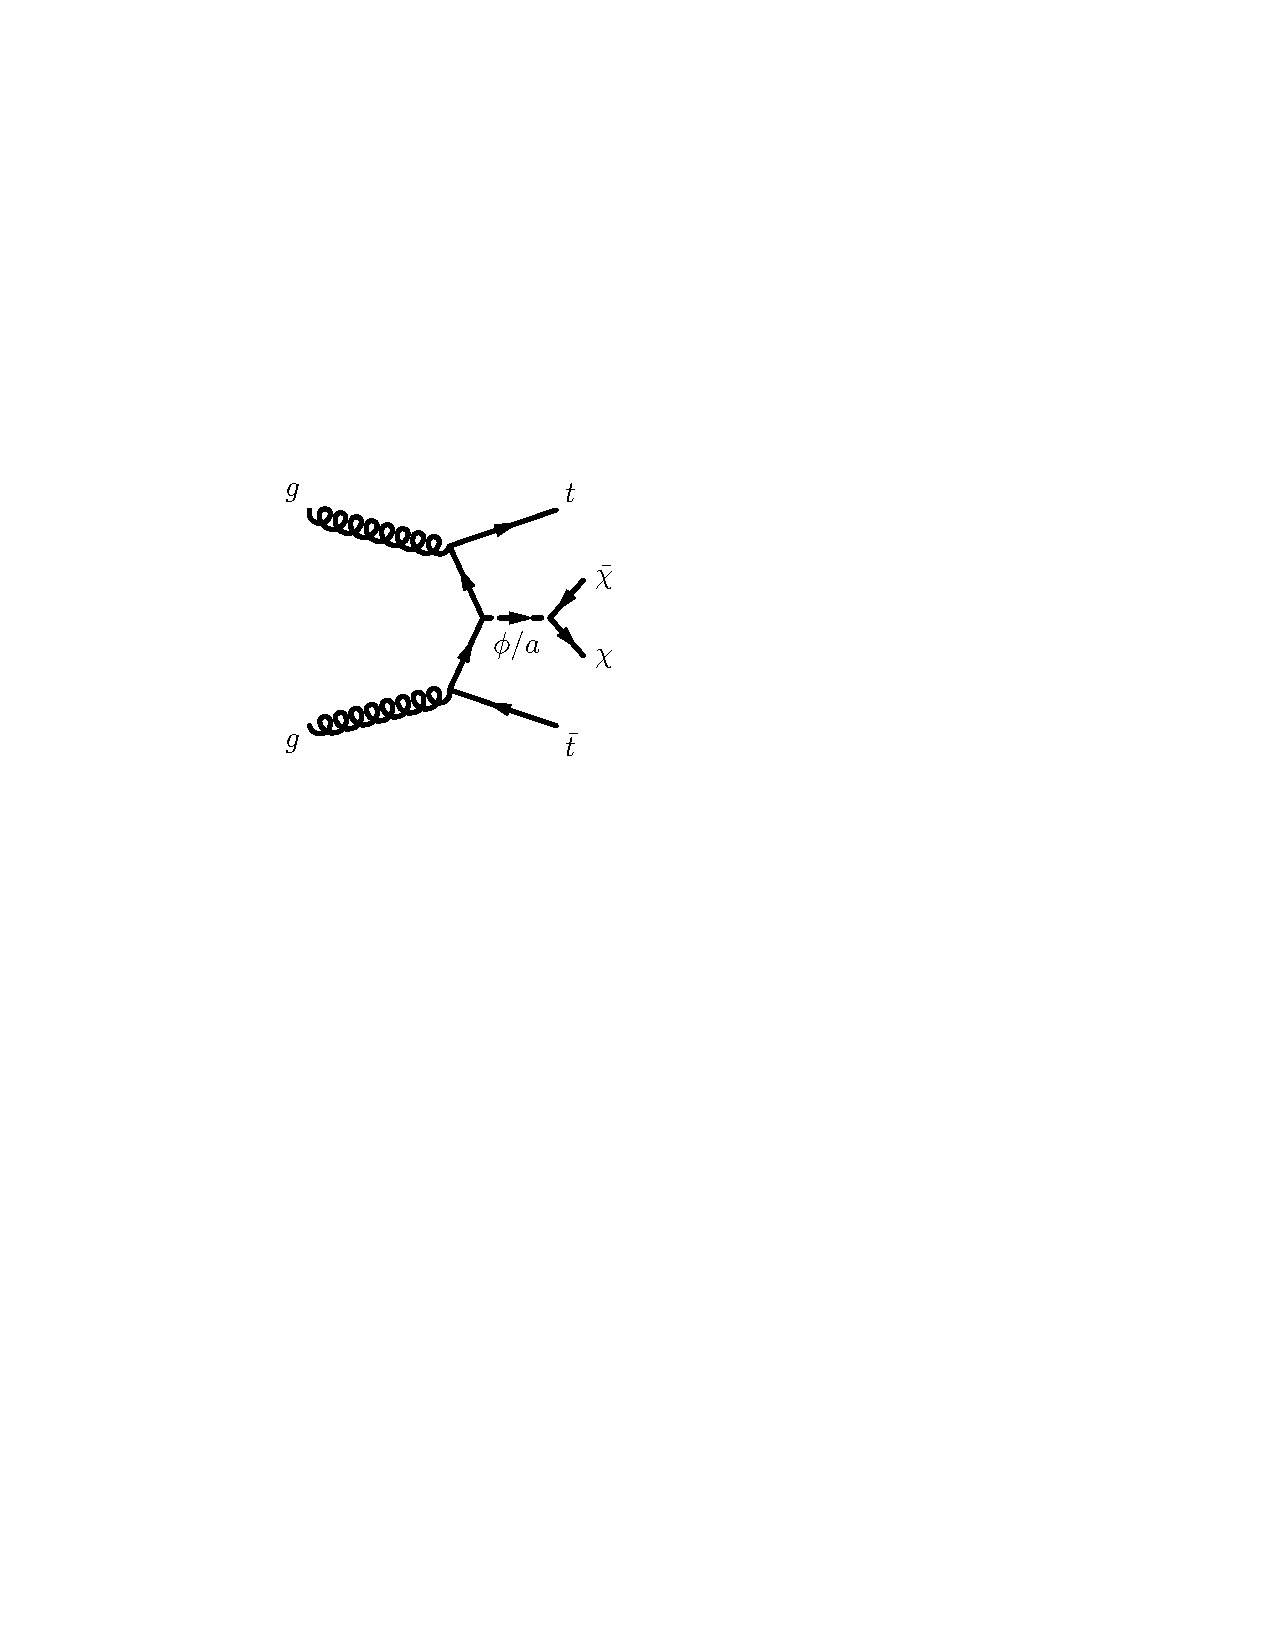
\includegraphics[width=.3\textwidth]{appA/TTphi}
		\caption{Representative diagrams at the lowest order for spin-0 mediator associated production with top quarks $\ttbar+\phi/a$ (taken from~\cite{DMhf})}
		\label{fig:dmhfModels}
	\end{wrapfigure}

	The data-driven background estimation technique and the theory uncertainties calculation prescription already discussed in Chapter~\ref{ch:stop_ana} were also employed in the search for dark matter produced in association with third-generation quarks, which was published in October 2017 in the \EPJ~\cite{DMhf}. This analysis also used $36.1\, \ifb$ of \pp\ collisions delivered by the \ac{LHC} and recorded with the \ac{ATLAS} detector, and although it targeted various final states with different number of leptons, depending on the \ttbar\ decay modes, the author's contribution was only used for the experimental signature shown in Figure~\ref{fig:dmhfModels}, as this is identical to the final states discussed in Chapter~\ref{ch:stop_ana}, namely the one shown in Figure~\ref{fig:stopModels}: 4 or more jets plus missing transverse momentum.

	The objects used, and the variables employed in the design of a region of control for the \ttgamma\ process, are the same as those used in the analysis already discussed in Chapter~\ref{ch:stop_ana}. Only one set of 2 \ac{SR} was used. Table bla shows the selection of the two \acp{SR}. 

	Table bla shows the control region selection employed (CR$\gamma$) to isolate the \ttgamma\ process. This essentially is identical to Table blabla already shown in Chapter~\ref{ch:stop_ana}. A purity of bla\% was reached and a scale factor of 1.whatever was obtained. 
	
	Figure bla2 shows the distribution of the \met\ in CR$\gamma$ where a very good data/MC agreement was found.
	
	The procedure adopted to estimate the contribution of the theory uncertainties to the total uncertainty is also the same and the results are shown in Table bla, where the highest uncertainty of whatever\% was obtained for SR bla. 
